\documentclass[10pt,twocolumn,letterpaper]{article}

\usepackage{ijcb}
\usepackage{times}
\usepackage{epsfig}
\usepackage{graphicx}
\usepackage{amsmath}
\usepackage{amssymb}
\usepackage{mathtools}
\usepackage{cite}
\usepackage{algpseudocode}
\usepackage[scientific-notation=true]{siunitx}


\usepackage{url}
\urldef{\mailsa}\path|thomas.bergmueller@authenticvision.com| 
\urldef{\mailsb}\path|uhl@cosy.sbg.ac.at|
\newcommand{\keywords}[1]{\par\addvspace\baselineskip
\noindent\keywordname\enspace\ignorespaces#1}



\providecommand{\myceil}[1]{\left \lceil #1 \right \rceil }
\providecommand{\myfloor}[1]{\left \lfloor #1 \right \rfloor }







% Include other packages here, before hyperref.

% If you comment hyperref and then uncomment it, you should delete
% egpaper.aux before re-running latex.  (Or just hit 'q' on the first latex
% run, let it finish, and you should be clear).
%\usepackage[pagebackref=true,breaklinks=true,letterpaper=true,colorlinks,bookmarks=false]{hyperref}

%\ijcbfinalcopy % *** Uncomment this line for the final submission

\def\ijcbPaperID{****} % *** Enter the IJCB Paper ID here
\def\httilde{\mbox{\tt\raisebox{-.5ex}{\symbol{126}}}}

% Pages are numbered in submission mode, and unnumbered in camera-ready
\ifijcbfinal\pagestyle{empty}\fi
\begin{document}

%%%%%%%%% TITLE
\title{\LaTeX\ Author Guidelines for IJCB 2014 Proceedings [Based on CVPR]}

\author{First Author\\
Institution1\\
Institution1 address\\
{\tt\small firstauthor@i1.org}
% For a paper whose authors are all at the same institution,
% omit the following lines up until the closing ``}''.
% Additional authors and addresses can be added with ``\and'',
% just like the second author.
% To save space, use either the email address or home page, not both
\and
Second Author\\
Institution2\\
First line of institution2 address\\
{\tt\small secondauthor@i2.org}
}

\maketitle
\thispagestyle{empty}

%%%%%%%%% ABSTRACT
\begin{abstract}
   Similar to the impact of aging on human beings, digital image sensors develop aging effects over time. Since these imager's aging effects (commonly denoted as pixel defects) leave marks in the captured images, it is not clear whether this affects the accuracy of iris recognition algorithms. This paper proposes a method to investigate the influence of sensor aging on iris recognition by simulative aging of an iris test database. A pixel model is introduced and an aging algorithm is discussed to create a test database. To establish practical relevance, the simulation parameters are obtained from the observed 4-year-aging effects of a real iris scanner.
\end{abstract}

%%%%%%%%% BODY TEXT



\section{Introduction}
% TODO probably start with a quote
The aging process starts immediately after being given birth. At first, aging's aspects are considered to be rather positive. One grows up, gets stronger and learns new things. At a certain point, aging starts to reveal several drawbacks. The skin gets wrinkled, joints and bones start to ache and also our vision starts to degenerate. In either case, aging changes parts of our body. Although human beings change, others are still able to recognize people they knew before, even when they haven't met in a long time and therefore aging changed their appearance significantly. \\
Biometric systems aim to identify human beings by analysing their biometric samples, i.e. the face, the fingerprints or iris \cite{rathgeb}. These systems operate in two steps. In the enrollment process, a subject's biometric samples are registered for the first time and stored in a database. Later, in the authentication procedure, another sample of a subject's biometric samples is taken and compared to the one stored in the database to verify the subject's identity. \\
Since there may be years or decades between the enrollment and the authentication, one strives to use biometric samples which are stable over time. The iris has widely been assumed to be stable, although it is currently topic of intensive discussion if and which iris-related information eventually changes in a human's aging process. Some researchers claim that iris-related information is stable or relatively stable \cite{daugmanPatent, daugmanNoChange, grotherStability, monroDCTIris}, while others observe significant changes over time \cite{rankinChange, rankinChangeResponse, fenkerIrisAging, czajkaTemplateAging, fairhurstNonstability}. Researchers mostly conclude these age-dependent changes in iris texture by observing changes in a system's iris-recognition rate. It is not clear, if observed changes in an algorithms' behaviour are caused by the aging of the tested subject, which is commonly assumed, aging of the recognition system itself or if this is caused by other unspecified factors.\\
This paper proposes a method to investitage the influence of aging effects of digital image sensors, which are crucial components of the recognition system. As a human being's vision often gets weaker with age, pixels start to get defective in image sensors over the years as well. This influences the quality - and therefore the appearance - of the captured images. Similar to being able to estimate a human being's age by his appearance, pixel defects observed in the captured images can reveal the age of the corresponding imager. This is used in image forensics to approximate the capturing date of an image \cite{fridrich}. However, since the aging effects of the sensor can be traced by evaluation of its output, namely the images, this implies that the capturing process is not time invariant. Hence two images, which capture the same (unchanged) scene, but were taken at significantly different points in time, may differ due to developed sensor defects in the meantime.
\\
\\ % TODO rephrase
There might arise problems due to sensor aging, because iris recognition systems operate by comparing current samples to earlier taken ones stored in a database. Special cameras with digital image sensors are commonly used to capture the iris features in both cases, the enrollment and the authentication process. It is not clear yet, whether the aging of the sensor - and thus the development of aging effects between taking two samples - influence the accuracy of iris recognition algorithms. To investigate this issue, one would need to have identical data captured at at least two significantly different points in time. It is practically impossible to establish identical conditions for both shots. Furthermore, as mentioned, it is not possible to distinguish between the influence of the subject's and the sensor's aging on iris recognition algorithms. For this reason one cannot capture test data to investigate the sensor's or the subject's aging in an isolated manner physically. There is no way to explicitely examine the iris texture's aging at all. However, it is possible to investigate the sensor aging's influence on the iris recognition rate independent from the subject's aging.\\
\\
%TODO Check Notredame for one sensor only
\textit{
We proposes a method to investigate the influence of a sensor's aging on the recognition rate. This is done by generating test data based on an the IITD iris database \cite{iitd} (TODO: Check if all captured by one sensor) by a simulated aging process. The practical relevance of this simulation is ensured by retrieving the simulation parameters from two iris databases 'NAME' \cite{agedIris}, where the same subjects were captured by the same sensor in 2009 and 2013. A method to retrieve the simulation parameters from this data is introduced in section \ref{hotPixelRate}. Using these simulation parameters, a pixel model and method to age images by generating images with hot and stuck pixels is discussed in \ref{virtualAging}. This test database is then used to test six implementations of iris recognition algorithms available in the University of Salzburg Iris Toolkit (USIT) \cite{usit} for influence of sensor aging effects upon the equal error rate (EER), refer section \ref{testing}. Finally we discuss the results and limitations of our tests (see section \ref{results}) and interpret them to give a statement about the influence of sensor aging on iris recognition algorithms in section \ref{conclusion}.}


\section{Sensor aging and pixel model}
An image sensor is a two dimensional array of photosensitive cells called pixels. The purpose of an image sensor is to convert the incoming light to its digital representation, which is commonly denoted as the image \cite{imageSensors}. In theory, each of these pixels has the same rectangular shape and a unified photo-response, meaning all pixels should produce the same output value on unified incoming light. Due to imperfections in the manufacturing process, this is not the case in practice, which means, there are pixels which are more sensitive than others \cite{camAndDisplays}. Besides that, some of a sensor's pixels might change their initial photo-response characteristic over the lifetime of a sensor. We denote this process of developing pixel defects over time as \emph{sensor aging}.   \\
Related work shows that such pixel defects caused by aging are equally distributed and independent throughout the sensor \cite{datingImages, inFieldDefects, defectDetection}. Furthermore, it is well known that the development of pixel defects linked to material-related faults is an increasing function of time \cite{failureSemi}. \\

\begin{figure}
\centering
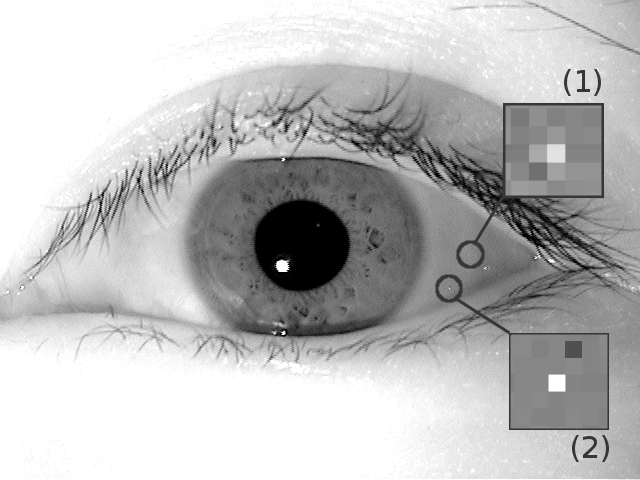
\includegraphics[height=5cm]{img/defects.png}
\caption{A \emph{partially-stuck pixel} (1) and two \emph{stuck pixels} (2) in an iris image. Contrast has been enhanced in the close-ups for visualisation. Note that the partially-stuck pixel still corresponds to the incoming light, but is significantly brighter compared to its neighbours, while the stuck pixel are light-independent and yield to a constant output.  }
\label{fig:hotStuck}
\end{figure}

The most common defects occuring over time are partially and fully stuck pixels, as shown in Fig. \ref{fig:hotStuck}. They are independent and uniformly distributed \cite{failureSemi, defectIdentification, fridrich}. Partially-stuck pixels tend to have a moderate offset compared to their neighbours, but still respond to the incident light, while stuck pixels always output a completely light-independent value and are often (but necessarily) saturated. As soon as a pixel is defective, it remains defective over the rest of the sensor's lifetime \cite{failureSemi}, regardless which type of defect it suffers. So one can obtain the important property that if a pixel is \emph{once defective, it remains defective}. This is illustrated in Fig. \ref{fig:defectLocations}.

\begin{figure}
\centering
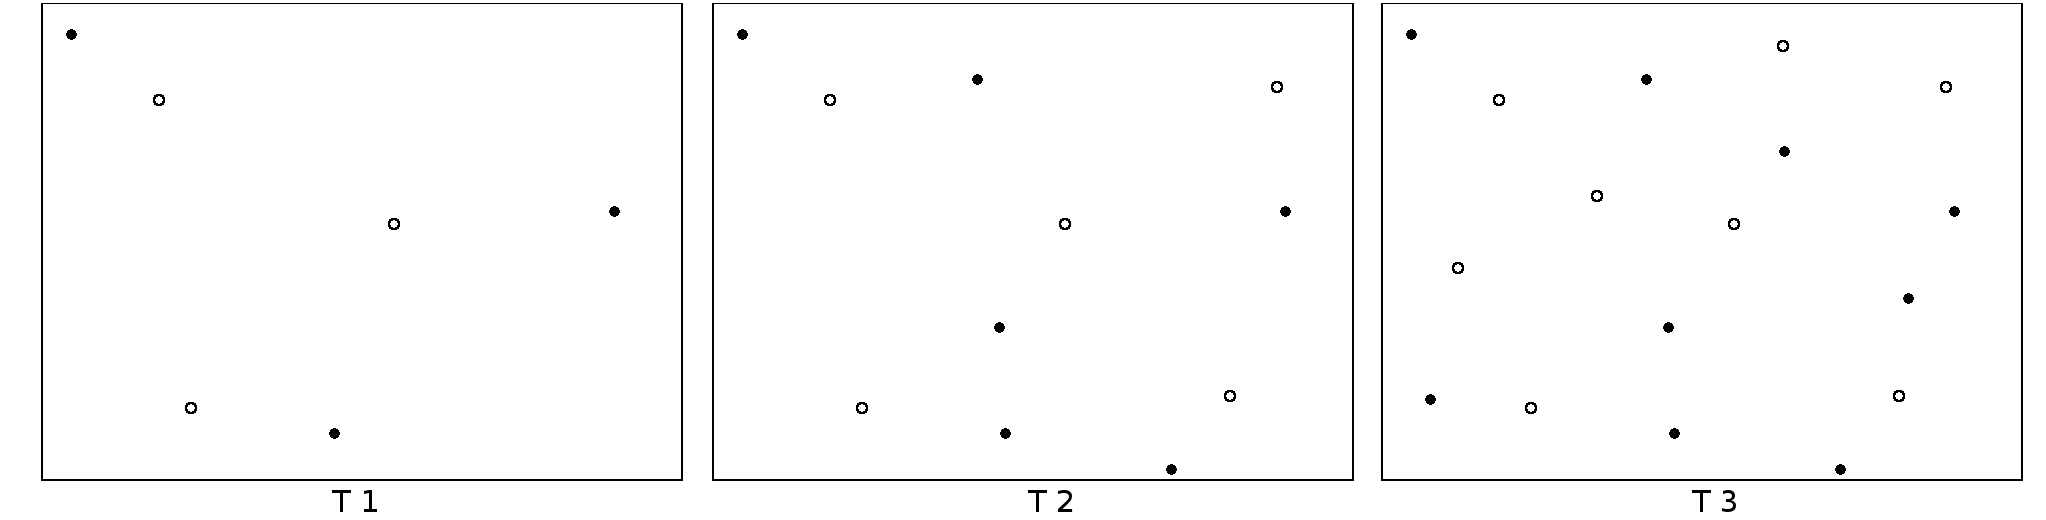
\includegraphics[width=\textwidth]{img/defectLocations.png}
\caption{Illustration of uniformly distributed and independent locations of partially-stuck (circle) and stuck (filled circle) pixels in images taken at 3 significantly different points in time T1, T2, T3.}
\label{fig:defectLocations}
\end{figure}

We conclude that the occurrence of new pixel defects can be modelled by a poisson process, while the location is uniformly distributed, hence randomly and independent. Already known defects remain constant in respect to their location and type \cite{fridrich, defectIdentification}. \\
\\
To run a simulation, a model for calculating the pixel values of an image $y$ has to be defined. There are several pixel output models around, which consider the incoming light and the impact of pixel defects on the raw output of a sensor. We denote $w,h \in \mathbb{Z}$ as the rows and columns of the sensor and start by adopting the model proposed in \cite{fridrich}:

\begin{equation}
\begin{aligned}
 Y = I+I \circ K+\tau D +c+\Theta \\ with \quad Y,I,K,D,C, \Theta \in \mathbb{R}^{w \times h}; \tau \in \mathbb{R}
\end{aligned}
  \label{equ:pixelmodel}
 \end{equation}

where $Y$ is the sensor output, commonly denoted as image, $I$ the intensity of incoming light, $I \circ K$ the photo-response non-uniformity PRNU, $\tau D$ the the dark current (with $\tau$ being a multiplicative-factor representing exposure settings, sensor temperature, \dots), $C$ a light-independent offset and $\Theta$ some modeling noise. Since all pixels are independent \cite{fridrich} \cite{defectDetection} and all operations element-wise, we denote the matrix-elements $y_{x,y} \in Y$ as $ y \in Y$ for simplicity reasons. The same applies to $i \in I$, $k \in K$, $d \in D$, $c \in C$ and $\theta \in \Theta$.\\
Since we're interested in simulating the aging effects of a specific sensor, all age-independent defects, which are e.g. due to production process, can be eliminated. Hence the PRNU, which corresponds to the non-uniformity of pixel-dimensions, can be omitted. As we're interested in reproducable tests, this means environmental influence (e.g. temperature) and modelling noise should be minimized. They can be eliminated completely in a simulation, thus we set $k=\theta=0$. Also the same exposure settings have to be used for the sensor in every test, therefore we have $\tau = const$ and set $ \tau = 1$ for simplicity. \cite{camAndDisplays}\cite{radiometricCCD}\cite{failureSemi}\cite{fridrich} suggest that the dark current is very weak with short exposure (which is necessary for applications in biometric systems to avoid motion blur). Under these considerations, a fairly simple model, considering only aging-relevant defects, remains:

\begin{equation}
  \label{equ:pixemodelEasier}
  y = i + d + c \quad with \quad y,i,c \in \mathbb{R}
\end{equation}

Common defect types that develop over time as the sensor ages are stuck and hot pixels, where the definitions of the latter are quite contrary in literature (e.g. in \cite{fridrich, defectIdentification, failureSemi}). If the dark current $d$ of a pixel is extremely high, this is often denoted as a hot pixel. If the offset $c$ is high, this results in a saturated pixel and is called a stuck pixel according to \cite{fridrich}. \cite{defectIdentification} suggests that a stuck pixel is not necessarily saturated but can obtain any value within the sensor output's universe. For the reason of non-uniform definitions of a hot pixel, we define the following models for defective pixels:

\begin{eqnarray}
     y & = & c \label{equ:Stuck} \\
  y & = & i + d \label{equ:Hot}
  \end{eqnarray}
  
where the defect in equ. \ref{equ:Stuck} is light-independent (thus referred as a \emph{stuck pixel}) and the defect in equ. \ref{equ:Hot} adds an offset and is commonly referred as either a partially-stuck or hot pixel. The dark current depends on exposure time and temperature, which both are kept constant this experiment. Thus also the dark current is constant and therefore there is no difference between a hot and a partially stuck pixel for this setup. We will denote this effect as a \emph{partially-stuck pixel}. In conclusion (and considering 8 bit grayscale images), the following pixel model is definied:

\begin{equation}
\begin{aligned}
Y_{x,y} = \begin{cases}
C_{x,y}  & \text{if $c_{x,y} \neq 0$}; \\
I_{x,y} +D_{x,y}  & \text{otherwise}.\\
\end{cases} \\ \text{with} \quad Y,C,I,D \in {(\mathbb{Z}:[0;255])}^{w \times h}
\label{equ:finalPixelModel}
\end{aligned} 
\end{equation}

where $Y_{x,y}$-values are clipped at $0$ and $255$ respectively if interval borders are exceeded, which means they saturate. 

\section{Simulated sensor aging}
\label{virtualAging}
For an ideal sensor, the defect matrices $C$ and $D$ are zero matrices. As pixel defects occur at a constant rate, this can be modelled by a poisson process \cite{fridrich}. Hence the number of stuck pixels and partially stuck pixels, denoted as $n_{s}$ and $n_{ps}$ respectively, at a specific point in time $t$ can be calculated as

\begin{eqnarray}
   n_s(t)  & = & t \lambda_s \\
  n_{ps}(t) & = &  t \lambda_{ps}
\end{eqnarray}

where $\lambda_s$ and $\lambda_{ps}$ are the rates at which the particular defect types occur. Due to defects being independent of each other, the location of the defect in the 2D sensor array can be modelled by a uniform distribution. Thus the defect location $(x,y)$ can be obtained using random numbers $r$. We propose the following procedure to obtain the position $s_k \in {w \times h}$ of the k-th pixel defect:

\begin{equation}
 s_k(x,y) = (\myfloor{\frac{r}{w}}, r \mod{w})) \quad \text{with} \quad r \in [0:w \cdot h]
\end{equation}

Depending on the k-th defect being a stuck or partially stuck pixel, the values of $C$ and $D$ according to the model defined in equ. \ref{equ:finalPixelModel} have to be set. We denote $a_s$ the maximum amplitude of a stuck pixel and $a_{ps}$ the maximum amplitude of a partially stuck pixel. Let $r_a \in \mathbb{R}:[0;1]$ be a uniformly distributed random number. Then we either have

\begin{eqnarray}
   C_{s_k}  & = & r_a \cdot a_s \quad \text{for stuck pixel at } s_k \text{ or} \\
   D_{s_k} & = &  r_a \cdot a_{ps} \quad \text{for partially stuck pixel at } s_k
\end{eqnarray}

These definitions together with the pixel model introduced in equ. \ref{equ:finalPixelModel} can be used to simulatively add aging-related sensor defects to an existing image $Y_{T_0}$ captured at time ${T_0}$. One might argue that $Y_{T_0}$ already contains pixel defects since the used sensor has defects at $T_0$ already. Since we are only interested in investigating if something changes over a period of time, it does not matter which time frame we observe. This means, already contained defects in $Y_{T_0}$ do not influence the outcome of the experiment. \\
Using the pixel model, sensor defects corresponding to a sensor's physical status at a specific time $T_i$ can be embedded in the image $Y_{T_0}$. The resulting image $Y_{T_i}$ can be interpreted as an image capturing the completely same scene as in $T_0$, but revealing the effects of sensor aging over a period of time $\Delta t = {T_i} - {T_0}$. Because sensor defects change over time, we define a sequence of defect matrices, which represent the state of aging at a specific point in time $T_i$. We denote these sequences corresponding to sample points $T_0$ \dots $T_m$ as

\begin{equation}
\begin{aligned}
(D_i)_{i=0..m} \text{ and } (C_i)_{i=0..m} \\ 
\text{with} \quad C_i, D_i \in {(\mathbb{Z}:[0;255])}^{w \times h}
\end{aligned}
\end{equation}
\\
By using them, we are able to simulate the physical state of the sensor at the considered sample points $T_0$ \dots $T_m$. To compute the sequence of aged images $Y_{T_1}$ \dots $Y_{T_m}$ from a source image $Y_{T_0}$, we define the following algorithm:
\\

\begin{algorithmic}[1]

\Procedure{AgedImageSequence}{$Y_{T_0}$}

\For{$i=1 \dots m$}
\State $\Delta t = T_i - T_0 $
\State $\Delta n_s\gets n_s(T_i - T_0) - n_s(T_{i-1} - T_0) $ 
\State $\Delta n_{ps}\gets n_{ps}(T_i - T_0) - n_{ps}(T_{i-1} - T_0) $
\State $D_i$ = $D_{i-1}$
\State $C_i$ = $C_{i-1}$

  \For{$k=1 \dots \Delta n_s$}
    \State $r_a \gets$ random in $[0;1]$
    \State $s_k \gets$ random in $w \times h$
    \State $C_{s_k} \gets r_a \cdot a_s$
  \EndFor
  
  \For{$k=1 \dots \Delta n_{ps}$}
    \State $r_a \gets$ random in $[0;1]$
    \State $s_k \gets$ random in $w \times h$
    \State $D_{s_k} \gets r_a \cdot a_{ps}$
  \EndFor
  
  
  $Y_{T_{i_{x,y}}} = \begin{cases}
  C_{i_{x,y}}  & \text{if $C_{i_{x,y}} \neq 0$}; \\
  Y_{T_{0_{x,y}}} +D_{i_{x,y}}  & \text{otherwise}.
  \end{cases}$
  
\EndFor
\State \textbf{return} $(Y_{T_i})_{i=1 \dots m}$
\EndProcedure
\end{algorithmic}


Basically for each point in time the number of defects-to-add $\Delta n_s, \Delta n_{ps}$ are calculated. The defect matrices $D$ and $C$ are computed recursively. This is necessary to satisfy the \emph{once defective, always defective} condition. By recursive calculation the earlier developed defects are persistent over virtual age. As soon as the defects for the $i$-th aging step are defined, they are used to compute an simulative aged image $Y_{T_i}$ using the pixel model defined in equ. \ref{equ:finalPixelModel}. Instead of the incident light $I$, the base image $Y_{T_0}$ can be used due to the previously given arguments. At the end we have a sequence  $(Y_{T_i})_{i=1 \dots m}$, where each element shows the scene captured in $Y_{T_0}$. Additionally each element $Y_i$ also contains the age-dependent defects of a sensor for a specific point in time $T_i$.

 
 \subsection{Finding simulation parameters from real sensor data (Rephrase)}
 \label{hotPixelRate}
 For the discussed simulation process, the defect's growth rate and amplitudes have to be defined. In laboratory set-ups hot and \emph{partially stuck pixels} are usually identified by dark calibration tests (i.e. $I=0$) \cite{defectIdentification}. To the best of the authors' knowledge, there is no such laboratory-captured data set available for iris imagers. There are databases \cite{czajkaTemplateAging, agedIris} available, which were captured using the same equipment for the purpose of investigating iris texture aging. In the following we propose a method to retrieve the growth rate and amplitudes of partially and fully stuck pixels from such databases.
 \\
TODO Luca:
\begin{itemize}
 \item I'd call this paragraph 'Relevance of the used database'
 \item Introduce database (``release note'')
 \item Argue relevance of data base (one sensor only) ... 
 \item Mention methods of prove why they are really from the same sensor (pls use BibTex-References)
\end{itemize}

For the simulation pixel model defined in equ. \ref{equ:finalPixelModel}, the growth rate and amplitudes of partially and fully stuck pixels have to be detected. As discussed, this type of defect is usually from a single image, incident light I is simply set to an uniform and known value, i.e. $I=0$. Hence only the defects $\Xi = D+C = Y-I$ remain. Because in our database $I$ is unknown statistics is used.
We denote $Y_0 \dots Y_K$ a sequence of $K$ images taken in a very short period of time. We know that a sensor defect has to be contained in each of this image and is (according to equ. \ref{equ:finalPixelModel}) independent of $I$. A \emph{stuck pixel} obtains the same value in each image in this sequence. Hence a pixel $y \in Y$ at position $(x,y)$ is identified as being stuck iff

\begin{equation}
y_{0} = y_{1} = \dots = y_{K} \label{equ:conditionStuck}
\end{equation}

To find partially stuck pixels, we compute the pixel's mean $\bar{y}$ from this sequence:
\begin{eqnarray}
\bar{y} & = & \frac{1}{K}\sum\limits_{k=1}^{K}y_k \\
\bar{y} & = & \frac{1}{K}\sum\limits_{k=1}^{K}(y_k+d+\theta_k) \label{equ:modelWithNoise} \\
\bar{y} & = & d+\frac{1}{K}\sum\limits_{k=1}^{K}(y_k) \label{equ:modelWithD}
\end{eqnarray}

Equ. \ref{equ:modelWithNoise} is obtained by using the pixel model of equ. \ref{equ:finalPixelModel} (without $c$, because stuck pixels fulfilling equ. \ref{equ:conditionStuck} are ignored in this process) and adding some modelling noise $\theta$. Since $d$ is a defect and therefore contained in every image in te sequence, it is independent of k. The mean of a uniformly distributed modelling noise $\theta$ cancels out for sufficiently large K. So we get equ. \ref{equ:modelWithD}.
The mean $\bar{y}$ tends to be the same for pixels within a local neighbourhood with maximum distance $q$ around $y$. This is the case if these pixels $Y_{{x \pm q, y \pm q}}$ had the same value in each image or their values had been uniformly distributed. When computing the median value of pixels in this $q$-neighbourhood, we again get $med(y,q) = \bar{y}$, even if one (but less than half) of the values is significantly different. Hence sparse pixel defects, which contribute to the mean, disappear when applying median filtering on the mean image. Considering only parts of the image, where mostly unified brightness and texture is present in $Y_1 \dots Y_K$ (refer fig. \ref{fig:correlated}), we conclude:
% TODO: q soll groß sein, wegen PRNU

\begin{eqnarray}
med(\bar{y},q) = d+\frac{1}{K}\sum\limits_{k=1}^{K}(y_k) \\
d = \frac{1}{K}\sum\limits_{k=1}^{K}y_k - med(\bar{y},q)
\end{eqnarray}
\begin{figure}
\centering
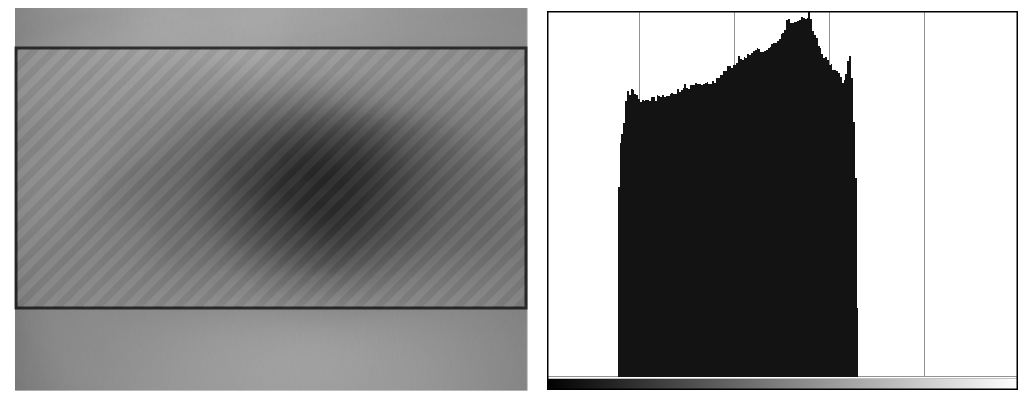
\includegraphics[width=\linewidth]{img/correlated.png}
\caption{The mean image of $Y_1 \dots Y_k$ has correlated data in the image's centre because of the iris usually being there. In the outer regions (marked), in almost all images skin and eyeball is captured in these regions, which tend to have unified brightness levels and little texture.}
\label{fig:correlated}
\end{figure}

\begin{figure}
\centering
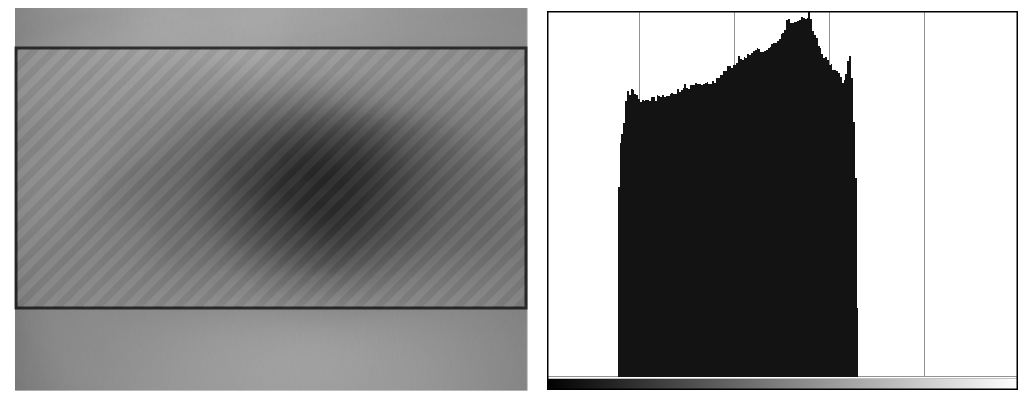
\includegraphics[width=\linewidth]{img/correlated.png}
\caption{Correctly classified pixel defects from $T_1$ are contained in $T_2$ as well. All other detected defects in $T_1$ can be interpreted as misclassification, since they violate the \emph{once defective, always defective}-condition}
\label{fig:defectPersistence}
\end{figure}
We declare a pixel to be partially stuck if $d$ exceeds a certain threshold $d > \tau_{ps}$. Since there is no reasonable way to find a optimal value for $\tau_{ps}$, we exploit the \emph{once defective, always defective}-property. We know, that a sensor's partially stuck pixels from $T_1$ also have to be present (along with others) in $T_2$. This is illustrated in fig. \ref{fig:defectPersistence}. By considering the number of defects $n_{match}$, which are present at the same location at $T_1$ and $T_2$ and the number of defects $n_1$ at $T_1$, the correctness ratio $s$ of the algorithm can be defined as
\begin{equation}
s = \frac{n_{match}}{n_1}
\end{equation}



Assuming that for $T_1$ and $T_2$ the same error is made, the observed increase of defects can be corrected by this factor $s$. With these observations and considering the size of a sensor $w\cdot h$, we retrieve the simulation parameters as \\

\begin{tabular}{l l l }
Param & Formula & from \cite{agedIris} \\
\hline 
$\lambda_{ps}$ & $s \cdot \frac{n_2-n_1}{(T_2-T_1)*(w \cdot h)}$ & $\lambda_{h100}=\num{1234}\frac{1}{1000 \text{px} \cdot \text{year}}$ \\ 
$\lambda_{s}$ & $s \cdot \frac{n_{s2}-n_{s1}}{(T_2-T_1)*(w \cdot h)}$ & $\lambda_{s} = 0$ \\
$ a_{ps}$ & $max(D)$ & $a_{ps_{h100}} = 3$ \\
$ a_{s}$ & $a_s := 255$ & $a_{s} = 255$ \\
\label{tab:parameters}
\end{tabular}

The retrieved values seem to correspond with the findings of other researchers, such as in \cite{defectDetection, leung}. Dudas \emph{et al} suggests in \cite{inFieldDefects} that real stuck pixels are never detected in field, because they are easy to detect at fabrication time (if any) or may correspond to partially stuck pixels with extremely high offset. However, we modelled real stuck pixels at a moderate growth rate (refer tab. \ref{tab:tests}) to investigate the influence if it happens stuck pixels occur. Furthermore, we modelled other sensors with growth rates retrieved from literature.




 \section{Testing}
 \label{testing}
 
 Other sources:
 \begin{itemize}
 \item $\lambda_{APS} = \num{0.000743423}$ from \cite{leung}
 \item $\lambda_{CCD} = \num{0.000569}$ from \cite{leung} 
 \item $\lambda_{h100}$ $\lambda_{oki}$ 
 \item $a_{ps_{h100}} = 3$ from experiment
 \item $a_{ps_{oki}} = ?$ from experiment
 
 \end{itemize}

 
 
 \begin{tabular}{c c c c }
 Sensor & $\lambda_{ps}$ & $\lambda_{s}$ & $a_{ps}$  \\
 \hline
 A	&	$\lambda_{h100}$ & 0.0 & $a_{ps_{h100}}$ \\
 B	&	$\lambda_{oki}$	& 0.0	& $a_{ps_{oki}}$   \\
 C & $\lambda_{h100}$ & $\lambda_{APS}$ & $a_{ps_{h100}}$ \\
 D & $\lambda_{oki}$ & $\lambda_{APS}$ & $a_{ps_{oki}}$    \\
 E & $\lambda_{APS}$ & 0 & $a_{ps_{h100}}$    \\
 F & $\lambda_{CCD}$ & 0 & $a_{ps_{h100}}$   \\
 G & 0 & $\lambda_{APS}$ & -- \\
 H & $ 4 \lambda_{h100}$ & 0 & $ 2 a_{ps_{h100}}$ \\
 I & $ 4 \lambda_{h100}$ & 0 & 100 \\
 J & $ 8 \lambda_{h100}$ &  $ 5 \lambda_{APS}$ & 100 \\
 \label{tab:tests}
 \end{tabular}
 
 
 
 \begin{itemize}
 \item Illustration of Locations in aged images + Amplitudes
 \item Argue that also stuck pixels are simulated at equal growth rate as partially stuck - although this is not observed in real data
 \item Argue tests with up to 8-times growth rate to cover also ``bad'' sensors
\end{itemize}
 
 
 \section{Results}
 \label{results}
 \subsection{Limitation of the results}
 \begin{itemize}
  \item Only one sensor tested (probably not representative)
  \item In-Camera fixing of sensor defects neglected (might influence development rate, but not so important, because also tested with multiples of the original rate)
  \item unsure whether noise reduction on in iris sensors
  \item But proved in JLEUNG that was off... so these rates probably representative
 \end{itemize}
 
 \section{Conclusion}
 \label{conclusion}
 TODO
 \begin{itemize}
  \item No influence of sensor aging found per se.
  \item Backs up the guys who claim that iris texture aging is really relevant and CAN be retrieved by observing influence on recognition rate
  \item TODO: Discuss conclusion with Mr. Uhl 
 \end{itemize}

 \section{Future work}
 \begin{itemize}
  \item Detect hot/stuck pixels by laboratory measurements. Compare to the observed method
  \item Also no true stuck pixel http://euler.ecs.umass.edu/research/ctkk-spie-2013.pdf
 \end{itemize}


% ------------------------ Reference section

{\small
\bibliographystyle{ieee}
\bibliography{egbib}
}

\end{document}
